\section{Exposure, self-calibration, and finite-data staging}
\label{sec:detectability}

\subsection{Exposure cannot cure exact alignment}

Let exposure $E$ scale both science and unconstrained nuisance scores as
\begin{equation}
 \bm s_E=\sqrt E\,\bm s,
 \qquad J_E=\sqrt E\,J.
\end{equation}
If $\bm s=J\bm a$ for some $\bm a$, then $\bm s_E=J_E\bm a$ for every $E>0$, so Proposition 2 gives
\begin{equation}
 \mathcal I_\beta(E)=0\qquad\forall E>0.
\label{eq:exposureno}
\end{equation}
RQIR-STAT-001 checks this explicitly from $E=1$ through $10^6$. ``More data'' therefore does not resolve an exact unconstrained nuisance degeneracy; a new response direction or independent nuisance information is required.

When $\mathcal I_\beta>0$ and independent observations add Fisher information, the local Cram\'er--Rao scaling is
\begin{equation}
 \sigma_\beta\gtrsim [N\mathcal I_\beta]^{-1/2}.
\label{eq:cramerrao}
\end{equation}
Equation~\eqref{eq:cramerrao} is only a staging relation. Translating $N$ or $\mathcal I_\beta$ into physical apparatus resources belongs to Paper III.

\subsection{Two-band self-calibration}

A complementary example shows how response diversity can break a nuisance degeneracy without an external prior. Let the whitened science score and a relative spectral-tilt nuisance be
\begin{equation}
 \bm g=(g_2,g_4)^T,
 \qquad
 \bm t=(g_2,-g_4)^T.
\end{equation}
Profiling the tilt gives
\begin{align}
 \mathcal I_{\beta\mid t}
 &=\bm g^T\bm g-
 \frac{(\bm g^T\bm t)^2}{\bm t^T\bm t}\\
 &=\boxed{\displaystyle\frac{4g_2^2g_4^2}{g_2^2+g_4^2}}.
\label{eq:twoband}
\end{align}
For $(g_2,g_4)=(0.3,0.7)$, the raw Fisher is $0.58$ and the profiled value is
\begin{equation}
 \mathcal I_{\beta\mid t}=0.3041379310344828,
\end{equation}
so the retained fraction is $\rho_\beta=0.5243757431629014$.

\begin{figure}[t]
\centering
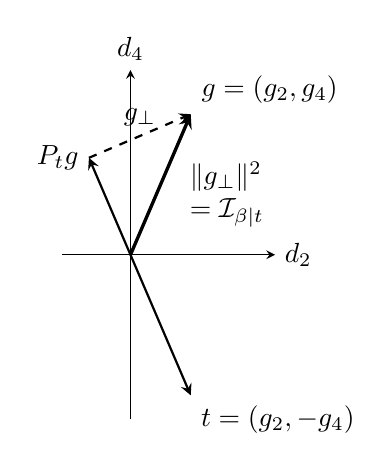
\begin{tikzpicture}[>=stealth,scale=2.55]
\draw[->] (-0.34,0) -- (0.72,0) node[right] {$d_2$};
\draw[->] (0,-0.82) -- (0,0.92) node[above] {$d_4$};
\coordinate (O) at (0,0);
\coordinate (G) at (0.30,0.70);
\coordinate (T) at (0.30,-0.70);
\coordinate (P) at (-0.2069,0.4828);
\draw[->,very thick] (O) -- (G) node[above right] {$\bm g=(g_2,g_4)$};
\draw[->,thick] (O) -- (T) node[below right] {$\bm t=(g_2,-g_4)$};
\draw[->,thick] (O) -- (P) node[left] {$P_t\bm g$};
\draw[->,thick,dashed] (P) -- (G) node[midway,above] {$\bm g_\perp$};
\node[align=left] at (0.48,0.30) {$\|\bm g_\perp\|^2$\\$=\mathcal I_{\beta\mid t}$};
\end{tikzpicture}

\caption{Whitened nuisance geometry for the two-band example. The target vector $\bm g$ is decomposed into a projection along the tilt nuisance and an orthogonal residual $\bm g_\perp$; the squared residual norm is the profiled Fisher information. The schematic geometry was AI-assisted and verified against Eq.~\eqref{eq:twoband}.}
\label{fig:geometry}
\end{figure}

Writing $r=g_4/g_2$, the retention becomes
\begin{equation}
 \rho_\beta(r)=\frac{4r^2}{(1+r^2)^2}.
\label{eq:rhoratio}
\end{equation}
It peaks at unity for balanced magnitudes $r=1$ and tends to zero when either band dominates. Thus ``adding a channel'' is not, by itself, the relevant statement; the new channel must rotate the science response relative to the nuisance span.

\begin{figure}[t]
\centering
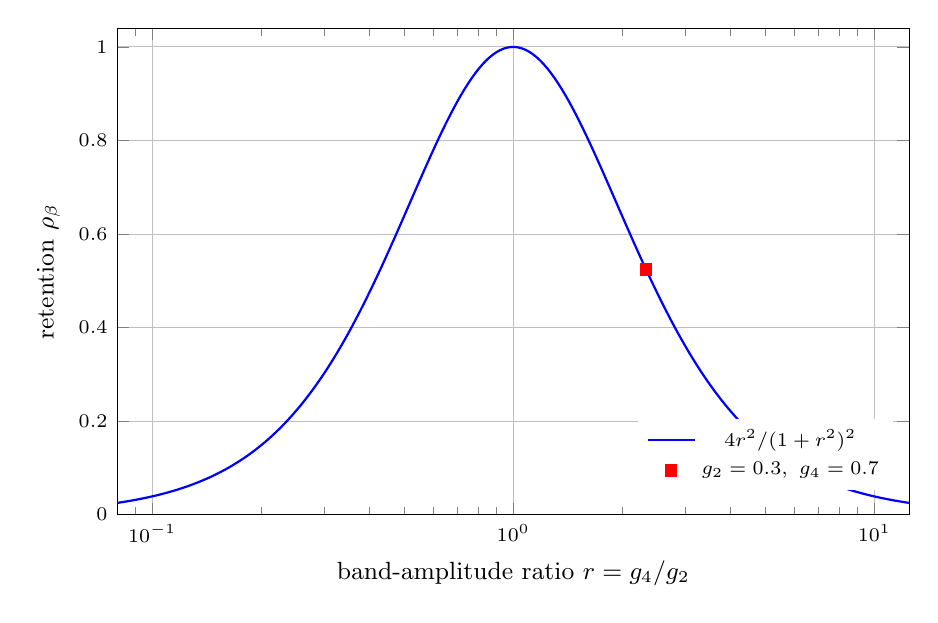
\begin{tikzpicture}
\begin{axis}[
 width=0.96\columnwidth,height=0.64\columnwidth,
 xmode=log,xmin=0.08,xmax=12.5,ymin=0,ymax=1.04,
 xlabel={band-amplitude ratio $r=g_4/g_2$},ylabel={retention $\rho_\beta$},
 grid=major,legend style={font=\scriptsize,draw=none,at={(0.98,0.05)},anchor=south east},
 tick label style={font=\scriptsize},label style={font=\small}]
\addplot[blue,thick,domain=0.08:12.5,samples=220] {4*x^2/(1+x^2)^2};
\addlegendentry{$4r^2/(1+r^2)^2$}
\addplot[only marks,mark=square*,red] coordinates {(2.3333333333,0.5243757431629014)};
\addlegendentry{$g_2=0.3,\ g_4=0.7$}
\end{axis}
\end{tikzpicture}

\caption{Two-band information retention, Eq.~\eqref{eq:rhoratio}. Balanced response gives complete local separation from the antisymmetric tilt nuisance, whereas strong band imbalance restores an approximate degeneracy. The marked RQIR-STAT-001 point retains about $52.44\%$ of the raw local Fisher information. Plotting code was AI-assisted and checked against archived curve data.}
\label{fig:retention}
\end{figure}

\subsection{A synthetic information-retention map}

To visualize the distinction between exact structural alignment, weak misalignment, and prior assistance, consider the normalized analytic family
\begin{equation}
 \bm s=(1,0)^T,\qquad
 \bm j=(1,\delta)^T,
\end{equation}
with scalar prior precision $\lambda\ge0$. Equation~\eqref{eq:priorfisher} gives
\begin{equation}
 \rho_\beta(\delta,\lambda)
 =\mathcal I_\beta(\delta,\lambda)
 =\frac{\delta^2+\lambda}{1+\delta^2+\lambda}.
\label{eq:map}
\end{equation}
The point $(0,0)$ is structurally degenerate; any nonzero $\delta$ creates data-only local identifiability, but the information can remain arbitrarily small. Nonzero $\lambda$ can instead supply prior-assisted precision even at $\delta=0$.

\begin{figure}[t]
\centering
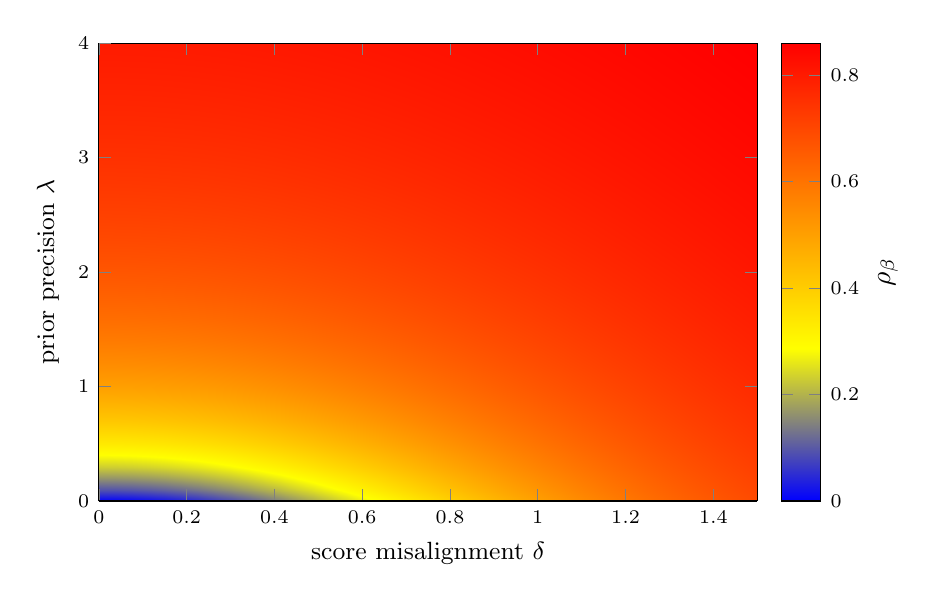
\begin{tikzpicture}
\begin{axis}[
 width=0.82\columnwidth,height=0.61\columnwidth,
 view={0}{90},xmin=0,xmax=1.5,ymin=0,ymax=4,
 xlabel={score misalignment $\delta$},ylabel={prior precision $\lambda$},
 colorbar,colorbar style={ylabel={$\rho_\beta$},yticklabel style={font=\scriptsize}},
 point meta min=0,point meta max=0.86,
 tick label style={font=\scriptsize},label style={font=\small}]
\addplot3[surf,shader=interp,domain=0:1.5,domain y=0:4,samples=41]
 {(x^2+y)/(1+x^2+y)};
\end{axis}
\end{tikzpicture}

\caption{Synthetic analytic information-retention map for Eq.~\eqref{eq:map}. The horizontal axis rotates the nuisance score away from exact alignment; the vertical axis adds independent nuisance precision. This is an identifiability diagnostic, not a physical reach forecast. Plotting code was AI-assisted and checked against archived grid data generated directly from Eq.~\eqref{eq:map}.}
\label{fig:map}
\end{figure}

\section{Shared and branch-specific nuisances}
\label{sec:branches}

Multiple detector branches or data subsets can share physical nuisance coefficients. The distinction between a genuinely shared nuisance and independent branchwise copies changes the nuisance subspace.

For independent data blocks $b=1,\ldots,B$, stack target scores and shared-nuisance matrices,
\begin{equation}
 \bm s=\begin{bmatrix}\bm s_1\\ \vdots\\ \bm s_B\end{bmatrix},
 \qquad
 J_{\rm sh}=\begin{bmatrix}J_1\\ \vdots\\ J_B\end{bmatrix}.
\end{equation}
If the same nuisance coefficient is instead allowed to vary independently in each branch, the nuisance matrix is
\begin{equation}
 J_{\rm sep}=\operatorname{diag}(J_1,\ldots,J_B).
\end{equation}

\paragraph*{Proposition 5 (shared-nuisance information bound).}
When the only difference is replacing one genuinely shared nuisance vector by unconstrained branch-specific copies,
\begin{equation}
 \mathcal I_{\rm shared}\ge \mathcal I_{\rm separate}.
\label{eq:sharedbound}
\end{equation}

\emph{Proof.} Every stacked displacement generated by a shared coefficient can also be generated by choosing equal branchwise copies, so
$\Col(J_{\rm sh})\subseteq\Col(J_{\rm sep})$ in the stacked data space. Proposition 3 then gives Eq.~\eqref{eq:sharedbound}. \hfill$\square$

The result is practically important: summing independently profiled branch Fishers is generally more conservative than a joint fit when the nuisance is truly shared. Conversely, imposing a shared nuisance without a physical justification can overstate information. The physical sharing structure must be declared before profiling.

\section{Correlated covariance and whitening invariance}
\label{sec:covariance}

For an unwhitened target derivative $\bm t$, nuisance matrix $K$, and positive-definite covariance $C$, the data-only profile is
\begin{equation}
 \mathcal I_\beta=
 \bm t^T C^{-1}\bm t
 -\bm t^T C^{-1}K
 (K^TC^{-1}K)^+
 K^TC^{-1}\bm t.
\label{eq:fullcov}
\end{equation}
Exact whitening by $C^{-1/2}$ maps Eq.~\eqref{eq:fullcov} to Eq.~\eqref{eq:schur}. Thus the geometry does not assume diagonal detector noise; it assumes only that the covariance used in the local reference likelihood is declared and positive definite on the retained data space.

As an additional submission-level regression beyond the historical seven-test certificate, we generated a deterministic correlated covariance with seed 20260908, dimension six, nuisance dimension two, and $\kappa(C)=21.4642$. Direct evaluation of Eq.~\eqref{eq:fullcov} gives $6.8036503258133445$; symmetric whitening gives $6.803650325813313$, an absolute difference $3.11\times10^{-14}$. The 10,000-trial stress audit described below found a maximum whitening discrepancy $5.97\times10^{-13}$ and no failures at tolerance $10^{-8}$.

\section{RQIR-STAT-001 deterministic reference certificate}
\label{sec:certificate}

The retained Paper-II science scope is frozen by the source-agnostic RQIR-STAT-001 reference-likelihood certificate. Its purpose is not to substitute for an apparatus model; it enforces algebraic invariants that any later detector likelihood must satisfy before resource calculations are credited. Table~\ref{tab:certificate} records an independent rerun against the current repository implementation.

\begin{table*}[t]
\caption{Submission rerun of the seven deterministic RQIR-STAT-001 regressions. All numbers were recomputed from the current certificate script with fixed seed 20260830. ``PASS'' means the stated analytic or invariant relation was satisfied at the certificate tolerance.}
\label{tab:certificate}
\begin{ruledtabular}
\begin{tabular}{p{0.20\textwidth}p{0.46\textwidth}p{0.23\textwidth}c}
Test & Invariant or expected result & Independent rerun & Status\\
\hline
A. Projection--Schur & $\mathcal I_\beta=\|(I-P_J)s\|^2$ & $1.1749239290799913$ vs. $1.1749239290799873$; $|\Delta|=4.00\times10^{-15}$ & PASS\\
B. Nuisance coordinates & $J\to JM$, $\Lambda\to M^T\Lambda M$ leaves $\mathcal I_\beta$ invariant & $1.8405965236299755$ vs. $1.8405965236299728$; $|\Delta|=2.66\times10^{-15}$ & PASS\\
C. Stronger nuisance information & $\Lambda_2-\Lambda_1\succeq0\Rightarrow \mathcal I_2\ge\mathcal I_1$ & $1.8405965236299755\to2.6370745801113067$ & PASS\\
D. Exact amplitude obstruction & $\mathcal I(C_a)=C_a/(1+C_a)$ & $C_a=9\to0.9$; all six stored values exact to tolerance & PASS\\
E. Exposure obstruction & exact alignment remains zero for any common exposure scaling & $E=1,2,10,100,10^6\to0$ & PASS\\
F. Two-band tilt & $4g_2^2g_4^2/(g_2^2+g_4^2)$ & $0.3041379310344828$ for $(0.3,0.7)$ & PASS\\
G. Rank-cutoff counterexample & true profile $\simeq0$; threshold deletion can return $1$ & $1.11\times10^{-16}$ vs. $1$ & PASS\\
\end{tabular}
\end{ruledtabular}
\end{table*}

These tests close several distinct failure modes. Tests A--C protect algebraic and coordinate consistency. Tests D and E distinguish an exact physical nuisance obstruction from low exposure. Test F demonstrates self-calibration by response diversity. Test G protects weak but physically aligned nuisance directions from arbitrary numerical deletion.

\section{Independent randomized stress audit}
\label{sec:stress}

A deterministic certificate can accidentally validate only its chosen examples. We therefore performed an independent property-based audit with seed 20260908 over 10,000 randomized problems. Data dimensions ranged from 4 to 11 and nuisance dimensions up to 4; every fifth trial was made intentionally rank deficient by replacing one nuisance column with an exact linear combination of the others. Separate random trials tested correlated positive-definite covariances.

The audit checked six properties: projection--Schur equality, nuisance-coordinate invariance with transformed priors, monotonicity under an added positive-semidefinite nuisance precision, exact-alignment collapse, the shared-nuisance bound, and full-covariance/whitening equivalence. No violation occurred at the declared tolerances. Table~\ref{tab:stress} reports the worst observed numerical discrepancies.

\begin{table}[t]
\caption{Independent 10,000-trial submission stress audit. The tolerances are deliberately looser than machine precision to accommodate ill-conditioned random coordinate changes; no trial exceeded them.}
\label{tab:stress}
\begin{ruledtabular}
\begin{tabular}{p{0.52\columnwidth}r}
Diagnostic & Worst or minimum value\\
\hline
max $|\mathcal I_{\rm Schur}-\mathcal I_{\rm proj}|$ & $1.31\times10^{-13}$\\
max nuisance-coordinate discrepancy & $1.02\times10^{-11}$\\
min stronger-prior gain & $2.13\times10^{-11}$\\
min $(\mathcal I_{\rm shared}-\mathcal I_{\rm separate})$ & $2.53\times10^{-7}$\\
max covariance-whitening discrepancy & $5.97\times10^{-13}$\\
violations in six property classes & $0$\\
\end{tabular}
\end{ruledtabular}
\end{table}

The randomized audit is a numerical robustness check, not a replacement for the analytic propositions. Its purpose is to detect implementation errors in rank-deficient, reparameterized, and correlated-covariance cases that are easy to miss with a single fixture.

The standalone submission-audit script used for this section was generated and debugged with substantive assistance from OpenAI ChatGPT (GPT-5.6 Sol). The executable outputs reported here were accepted only after comparison with the frozen deterministic certificate, direct analytic identities, and independent property checks with fixed seeds; the AI system was not used as a numerical authority.

\section{Numerical rank discipline: a minimal false-detection counterexample}
\label{sec:rank}

Pseudoinverse tolerances can change the physics if they are used to delete weak nuisance directions by norm alone. Consider
\begin{equation}
 \bm s=(1,0)^T,
 \qquad
 \bm j=(\epsilon,0)^T,
 \qquad \epsilon=10^{-8}.
\label{eq:cutoffcase}
\end{equation}
The nuisance norm is tiny, but its span is exactly the science direction. Exact geometric profiling therefore gives zero information, numerically $1.11\times10^{-16}$ in the stored floating-point calculation.

A bad implementation that discards the nuisance whenever $j^Tj\le\tau$ instead returns
\begin{equation}
 \mathcal I_{\rm bad}=1
\end{equation}
for any $\tau\ge10^{-16}$. In particular, the historical counterexample uses $\tau=10^{-12}$. The apparent ``detection'' is created entirely by a numerical cutoff.

\begin{figure}[t]
\centering
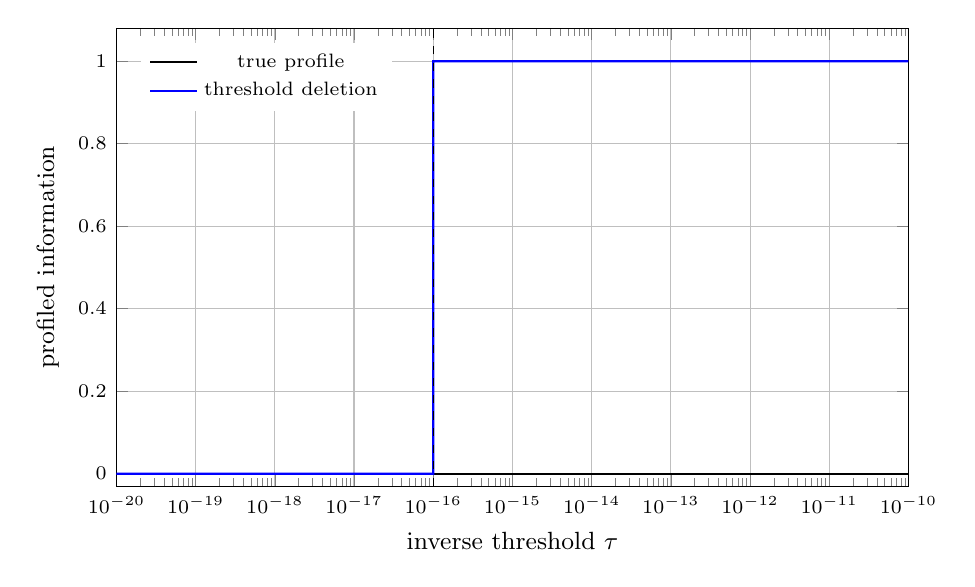
\begin{tikzpicture}
\begin{axis}[
 width=0.96\columnwidth,height=0.61\columnwidth,
 xmode=log,xmin=1e-20,xmax=1e-10,ymin=-0.03,ymax=1.08,
 xlabel={inverse threshold $\tau$},ylabel={profiled information},
 grid=major,legend style={font=\scriptsize,draw=none,at={(0.03,0.97)},anchor=north west},
 tick label style={font=\scriptsize},label style={font=\small}]
\addplot[black,thick] coordinates {(1e-20,0) (1e-10,0)};
\addlegendentry{true profile}
\addplot[blue,thick] coordinates {(1e-20,0) (9.99e-17,0) (1e-16,1) (1e-10,1)};
\addlegendentry{threshold deletion}
\addplot[dashed] coordinates {(1e-16,-0.03) (1e-16,1.08)};
\end{axis}
\end{tikzpicture}

\caption{RQIR-NUM-001 cutoff counterexample. The exact nuisance span is collinear with the science score for every nonzero $\epsilon$, so the true profile remains zero. A threshold-deletion implementation jumps discontinuously to unit information once the inverse cutoff exceeds $\epsilon^2=10^{-16}$. Plotting code was AI-assisted and checked against the analytic branch condition and archived scan data.}
\label{fig:cutoff}
\end{figure}

The methodological rule is therefore stronger than ``choose a small tolerance'': exact hard constraints should be eliminated analytically where possible, and weak physical nuisance directions must not be removed merely because their singular values are small. Numerical regularization must be justified relative to a physical prior, an explicit model reduction, or a demonstrated stability criterion.
